\subsection{奇异信号}

\subsubsection{单位斜变信号}

\begin{definition}[单位斜变信号]
    \bd{单位斜变信号}的数学表达式为
    \begin{align*}
        R(t) = \begin{cases}
            0, & t < 0, \\
            t, & t \ge 0.
        \end{cases}
    \end{align*}
    信号图像如图 \ref{fig:ramp-signal} 所示。
    \begin{figure}[H]
        \centering
        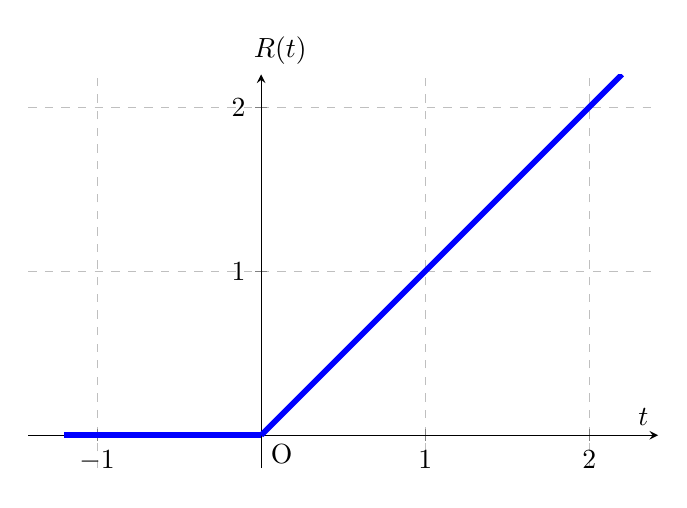
\begin{tikzpicture}
            \begin{axis}[
                axis lines = middle,
                xlabel = {$t$},
                ylabel = {$R(t)$},
                ylabel style={at={(rel axis cs:0.4, 1)}, anchor=south},
                xmin = -1.2, xmax = 2.2,
                ymin = -0.2, ymax = 2.2,
                xtick distance = 1,
                ytick distance = 1,
                grid = major,
                grid style = dashed,
                scale only axis,
                width = 8cm,
                height = 5cm,
                axis equal,
            ]
            \addplot[domain=-1.2:0, samples=100, smooth, line width=2pt, blue] {0};
            \addplot[domain=0:2.2, samples=100, smooth, line width=2pt, blue] {x};
            \node at (axis cs:0, 0) [anchor=north west] {O};
            \end{axis}
        \end{tikzpicture}
        \caption{单位斜变信号}
        \label{fig:ramp-signal}
    \end{figure}
\end{definition}

\begin{definition}[截顶的单位斜变信号]
    \bd{截顶的单位斜变信号}的数学表达式为
    \begin{align*}
        R_{\tau}(t) = \begin{cases}
            0, & t < 0, \\
            t, & 0 \le t \le \tau, \\
            \tau, & t > \tau.
        \end{cases}
    \end{align*}
    信号图像如图 \ref{fig:truncated-ramp-signal} 所示。
    \begin{figure}[H]
        \centering
        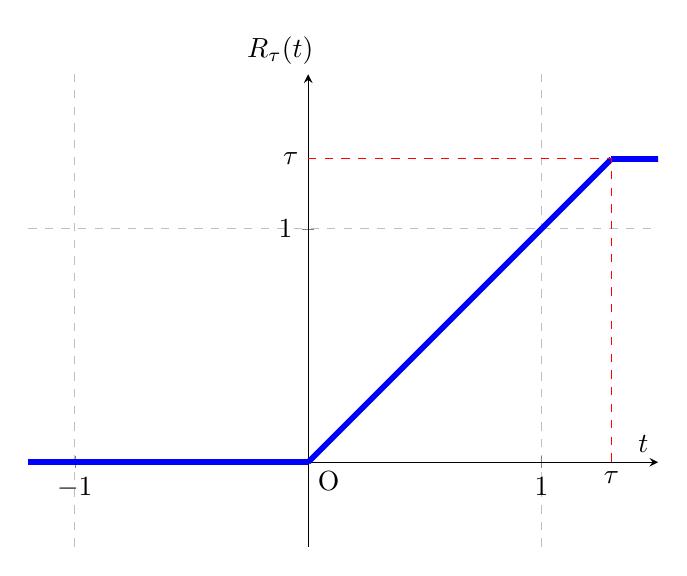
\begin{tikzpicture}
            \begin{axis}[
                axis lines = middle,
                xlabel = {$t$},
                ylabel = {$R_{\tau}(t)$},
                ylabel style={at={(rel axis cs:0.4, 1)}, anchor=south},
                xmin = -1.2, xmax = 1.5,
                ymin = -0.2, ymax = 1.5,
                xtick distance = 1,
                ytick distance = 1,
                grid = major,
                grid style = dashed,
                scale only axis,
                width = 8cm,
                height = 6cm,
                axis equal,
            ]
            \addplot[domain=-1.2:0, samples=100, smooth, line width=2pt, blue] {0};
            \addplot[domain=0:1.3, samples=100, smooth, line width=2pt, blue] {x};
            \addplot[domain=1.3:2.2, samples=100, smooth, line width=2pt, blue] {1.3};
            \addplot[dashed, red] coordinates {(0, 1.3) (1.3, 1.3) (1.3, 0)};
            \node at (axis cs:0, 0) [anchor=north west] {O};
            \node at (axis cs:0, 1.3) [anchor = east] {$\tau$};
            \node at (axis cs:1.3, 0) [anchor = north] {$\tau$};
            \end{axis}
        \end{tikzpicture}
        \caption{截顶的单位斜变信号}
        \label{fig:truncated-ramp-signal}
    \end{figure}
\end{definition}

\subsubsection{单位阶跃信号}

\begin{definition}[单位阶跃信号]
    \bd{单位阶跃信号}的数学表达式为
    \begin{align*}
        u(t) = \begin{cases}
            0, & t < 0, \\
            1, & t \ge 0.
        \end{cases}
    \end{align*}
    信号图像如图 \ref{fig:step-signal} 所示。
    \begin{figure}[H]
        \centering
        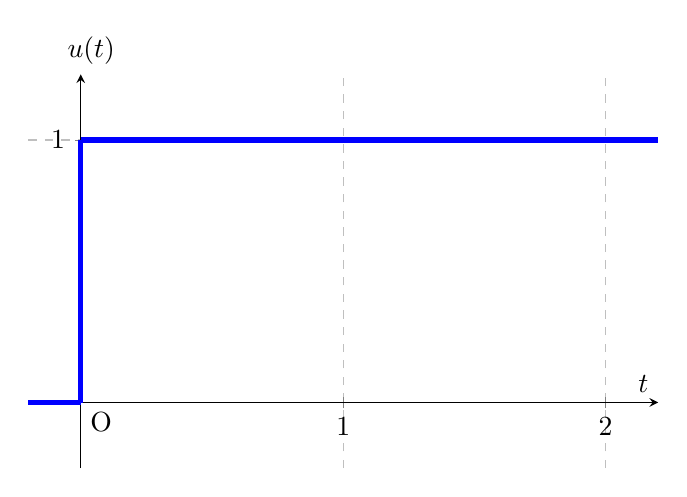
\begin{tikzpicture}
            \begin{axis}[
                axis lines = middle,
                xlabel = {$t$},
                ylabel = {$u(t)$},
                ylabel style={at={(rel axis cs:0.1, 1)}, anchor=south},
                xmin = -0.2, xmax = 2.2,
                ymin = -0.2, ymax = 1.2,
                xtick distance = 1,
                ytick distance = 1,
                grid = major,
                grid style = dashed,
                scale only axis,
                width = 8cm,
                height = 5cm,
                axis equal,
            ]
            \addplot[domain=-1.2:0, samples=100, smooth, line width=2pt, blue] {0};
            \addplot[smooth, line width=2pt, blue] coordinates {(0, 0) (0, 1)};
            \addplot[domain=0:2.2, samples=100, smooth, line width=2pt, blue] {1};
            \node at (axis cs:0, 0) [anchor=north west] {O};
            \end{axis}
        \end{tikzpicture}
        \caption{单位阶跃信号}
        \label{fig:step-signal}
    \end{figure}
\end{definition}

\begin{property}[单位阶跃信号与单位斜变信号的关系]
    单位斜变信号是单位阶跃信号的积分,即
    \begin{align*}
        R(t) = \int_{-\infty}^{t}u(\tau)\D{\tau}.
    \end{align*}
    单位阶跃信号是单位斜变信号的微分,即
    \begin{align*}
        u(t) = \frac{\D{R(t)}}{\D{t}}.
    \end{align*}
\end{property}

\subsubsection{单位矩形脉冲信号}

\begin{definition}[单位矩形脉冲信号]
    \bd{单位矩形脉冲信号}的数学表达式为
    \begin{align*}
        G_{\tau}(t) = \begin{cases}
            0, & \abs{t} \le \frac{\tau}{2}, \\
            1, & \abs{t} > \frac{\tau}{2}.
        \end{cases}
    \end{align*}
    信号图像如图 \ref{fig:rectangular-pulse-signal} 所示。
    \begin{figure}[H]
        \centering
        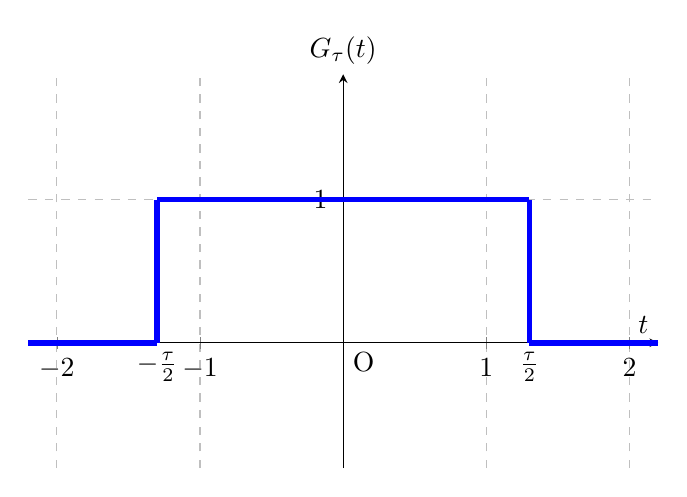
\begin{tikzpicture}
            \begin{axis}[
                axis lines = middle,
                xlabel = {$t$},
                ylabel = {$G_{\tau}(t)$},
                ylabel style={at={(rel axis cs:0.5, 1)}, anchor=south},
                xmin = -2.2, xmax = 2.2,
                ymin = -0.2, ymax = 1.2,
                xtick distance = 1,
                ytick distance = 1,
                grid = major,
                grid style = dashed,
                scale only axis,
                width = 8cm,
                height = 5cm,
                axis equal,
            ]
            \addplot[domain=-2.2:-1.3, samples=100, smooth, line width=2pt, blue] {0};
            \addplot[domain=-1.3:1.3, samples=100, smooth, line width=2pt, blue] {1};
            \addplot[domain=1.3:2.2, samples=100, smooth, line width=2pt, blue] {0};
            \addplot[smooth, line width=2pt, blue] coordinates {(-1.3, 0) (-1.3, 1)};
            \addplot[smooth, line width=2pt, blue] coordinates {(1.3, 1) (1.3, 0)};
            \node at (axis cs:0, 0) [anchor=north west] {O};
            \node at (axis cs:-1.3, 0) [anchor = north] {$-\frac{\tau}{2}$};
            \node at (axis cs:1.3, 0) [anchor = north] {$\frac{\tau}{2}$};
            \end{axis}
        \end{tikzpicture}
        \caption{单位矩形脉冲信号}
        \label{fig:rectangular-pulse-signal}
    \end{figure}
    其中,\bd{脉高}是指脉冲信号的高度,\bd{脉宽}是指脉冲信号的宽度。
\end{definition}

\begin{property}[单位矩形脉冲信号与单位阶跃信号的关系]
    单位矩形脉冲信号是两个单位阶跃信号的差,即
    \begin{align*}
        G_{\tau}(t) = u\left(t + \frac{\tau}{2}\right) - u\left(t - \frac{\tau}{2}\right).
    \end{align*}
\end{property}

\begin{remark}
    不必再用分段的形式来表示信号,可以使用矩形脉冲信号来表示。
    其他信号与矩形脉冲信号相乘时,只有在矩形脉冲信号对应的区间内,
    其他信号的信息才被保留下来,其余范围都是零。

    用矩形脉冲信号和乘法运算,可以截取信号的特定区间片段。
    所以,单位矩形脉冲信号也被称为``窗函数''。如图 \ref{fig:rectangular-pulse-signal-example} 所示。
    \begin{figure}[H]
        \centering
        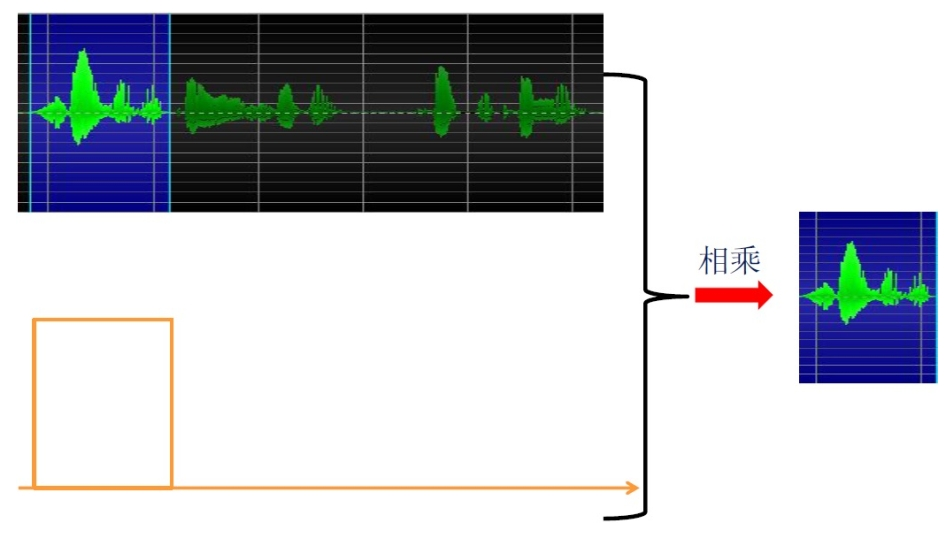
\includegraphics[width=0.5\textwidth]{chap1/img/rectangular-pulse-signal-example.png}
        \caption{窗函数的截取功能}
        \label{fig:rectangular-pulse-signal-example}
    \end{figure}
\end{remark}

\subsubsection{符号函数信号}

\begin{definition}[符号函数信号]
    \bd{符号函数信号}的数学表达式为
    \begin{align*}
        \sgn{t} = \begin{cases}
            -1, & t < 0, \\
            0, & t = 0, \\
            1, & t > 0.
        \end{cases}
    \end{align*}
    信号图像如图 \ref{fig:sign-signal} 所示。
    \begin{figure}[H]
        \centering
        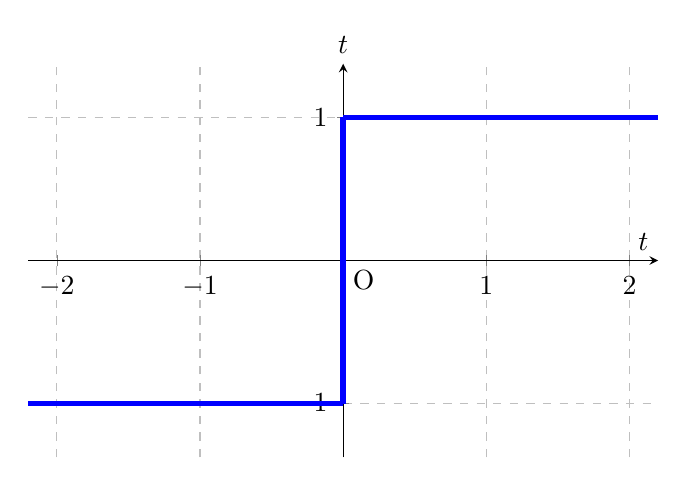
\begin{tikzpicture}
            \begin{axis}[
                axis lines = middle,
                xlabel = {$t$},
                ylabel = {$\sgn{t}$},
                ylabel style={at={(rel axis cs:0.5, 1)}, anchor=south},
                xmin = -2.2, xmax = 2.2,
                ymin = -1.2, ymax = 1.2,
                xtick distance = 1,
                ytick distance = 1,
                grid = major,
                grid style = dashed,
                scale only axis,
                width = 8cm,
                height = 5cm,
                axis equal,
            ]
            \addplot[domain=-2.2:0, samples=100, smooth, line width=2pt, blue] {-1};
            \addplot[domain=0:2.2, samples=100, smooth, line width=2pt, blue] {1};
            \addplot[smooth, line width=2pt, blue] coordinates {(0, -1) (0, 1)};
            \node at (axis cs:0, 0) [anchor=north west] {O};
            \end{axis}
        \end{tikzpicture}
        \caption{符号函数信号}
        \label{fig:sign-signal}
    \end{figure}
    符号函数信号通常用于表示自变量的符号特性。
\end{definition}

\begin{property}[符号函数信号与单位阶跃信号的关系]
    由 $\sgn{t} + 1 = 2u(t)$ 可得,
    \begin{align*}
        \sgn{t} = 2u(t) - 1.
    \end{align*}
\end{property}

\subsubsection{单位冲激信号}

\begin{definition}[单位冲激信号的狄拉克定义式]
    设冲激信号有一个总的冲激强度,它在整个时间域上的积分等于该强度值,
    而在除冲激点之外的其他点的函数取值为零。
    定义\bd{单位冲激信号}$\delta(t)$ 为满足以下条件的信号:
    \begin{align*}
        \begin{cases}
            \int_{-\infty}^{+\infty}\delta(t)\D{t} = 1, \\
            \delta(t) = 0 \quad (t \neq t_0).
        \end{cases}
    \end{align*}
    这也被称为 $\delta(t)$ 的狄拉克定义式。
    更一般地,可以定义冲激点在 $t_0$,强度为 $E$ 的冲激信号为
    \begin{align*}
        \delta_{E, t_0}(t) = E \cdot \delta(t - t_0),
    \end{align*}
    它满足
    \begin{align*}
        \begin{cases}
            \int_{-\infty}^{+\infty}\delta_{E, t_0}(t)\D{t} = E, \\
            \delta_{E, t_0}(t) = 0 \quad (t \neq t_0).
        \end{cases}
    \end{align*}

    信号图像如图 \ref{fig:impulse-signal} 所示。
    在冲激点处画一条带箭头的线,线的方向和长度与冲激强度的符号和大小一致。
    \begin{figure}[H]
        \centering
        \begin{tikzpicture}
            \begin{axis}[
                axis lines = middle,
                xlabel = {$t$},
                ylabel = {$\delta(t)$},
                ylabel style={at={(rel axis cs:0.5, 1)}, anchor=south},
                xmin = -0.2, xmax = 2.2,
                ymin = -0.2, ymax = 2.2,
                xtick distance = 1,
                ytick distance = 1,
                grid = major,
                grid style = dashed,
                scale only axis,
                width = 6cm,
                height = 5cm,
                axis equal,
            ]
            \draw[-stealth, smooth, red] (axis cs:1.3, 0) -- (axis cs:1.3, 1.5);
            \node at (axis cs:0, 0) [anchor=north west] {O};
            \node at (axis cs:1.3, 0) [anchor=north] {$t_0$};
            \node at (axis cs:1.3, 1.5) [anchor=west] {$(E)$};
            \end{axis}
        \end{tikzpicture}
        \caption{单位冲激信号}
        \label{fig:impulse-signal}
    \end{figure}

    单位冲激信号通常用于描述自然界中那些发生后持续时间很短的现象。
\end{definition}

\begin{definition}[单位冲激信号的极限定义式]
    设 $G_{\tau}(t)$ 是一个单位矩形脉冲信号,其脉宽为 $\tau$,则
    \begin{align*}
        \delta(t) = \lim_{\tau \to 0}\frac{G_{\tau}(t)}{\tau},
    \end{align*}
    即单位冲激信号是单位矩形脉冲信号的极限。
\end{definition}

\begin{remark}
    更一般地,设位于 $[-\frac{\tau}{2}, \frac{\tau}{2}]$ 上的
    信号 $f_{\tau}(t)$ 的脉冲宽度为 $\tau$,若能保证
    \begin{align*}
        \int_{-\frac{\tau}{2}}^{\frac{\tau}{2}}f_{\tau}(t)\D{t} = 1, \quad \forall \tau > 0,
    \end{align*}
    即始终保持单位面积,则
    \begin{align*}
        \delta(t) = \lim_{\tau \to 0}f_{\tau}(t),
    \end{align*}
    即单位冲激信号是信号 $f_{\tau}(t)$ 的极限。$f_{\tau}(t)$ 可以是矩形脉冲、三角脉冲等。
\end{remark}

\begin{property}[冲激函数的搬移抽样特性]
    对于任意的信号 $f(t)$ 而言,都有 $f(t) * \delta(t) = f(t)$。
    更一般地,一个函数与单位冲激函数的卷积,等价于把该函数平移到
    单位冲激函数的冲激点位置,即
    \begin{align*}
        f(t) * \delta(t - t_0) = f(t - t_0),
    \end{align*}
    运算前后的信号如图 \ref{fig:impulse-signal-convolution-translation} 所示。
    \begin{figure}[H]
        \centering
        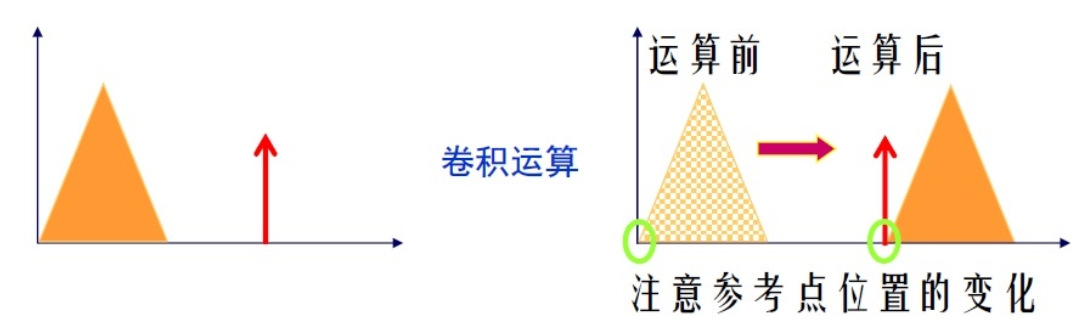
\includegraphics[width=0.5\textwidth]{chap1/img/impulse-signal-convolution-translation.png}
        \caption{冲激函数的搬移抽样特性}
        \label{fig:impulse-signal-convolution-translation}
    \end{figure}
\end{property}

\begin{proof}
    \begin{align*}
        f(t) * \delta(t - t_0) = \int_{-\infty}^{+\infty}f(a)\delta(t - t_0 - a)\D{a},
    \end{align*}
    而 $\delta(t - t_0 - a)$ 只有在 $a = t - t_0$ 时非零。因此
    \begin{align*}
        f(t) * \delta(t - t_0) & = \int_{-\infty}^{+\infty}f(t - t_0)\delta(t - t_0 - a)\D{a} \\
        & = f(t - t_0)\int_{-\infty}^{+\infty}\delta(t - t_0 - a)\D{a} \\
        & = f(t - t_0).
    \end{align*}
\end{proof}

\begin{property}[从函数到值的映射关系]
    冲激函数能从检验函数中筛选出零点处的函数值。对于任意的函数 $f(t)$,有
    \begin{align*}
        \int_{-\infty}^{+\infty}f(t)\delta(t)\D{t} = f(0).
    \end{align*}

    上式只是借用了积分的形式,表达的意思是:冲激函数对测试函数分配(或赋予)一个数的过程,
    所以不能按普通的积分运算来考虑。
    之所以借用积分的形式,是因为它形式上与积分运算的相应性质一致,
    且普通积分运算实际上也是产生一个``值''。
\end{property}

\begin{property}[冲激函数的性质总结]
    冲激函数 $\delta(t)$ 具有以下性质:
    \begin{enumerate}
        \item (对称性) $\delta(t)$ 为偶函数,即 $\delta(t) = \delta(-t)$。
        \item (时域压扩性) $\delta(at) = \frac{1}{\abs{a}}\delta(t), a \neq 0$。
        \item (积分) 积分值为 $1$ 还是 $0$,取决于积分区间是否包含原点,即:
            \begin{align*}
                \begin{cases}
                    \int_{-\infty}^{t}\delta(\tau)\D{\tau} = 1, & t > 0, \\
                    \int_{-\infty}^{t}\delta(\tau)\D{\tau} = 0, & t < 0.
                \end{cases}
            \end{align*}
            即:$\int_{-\infty}^{t}\delta(\tau)\D{\tau} = u(t)$。
            单位冲激函数的积分是单位阶跃函数。
        \item (抽样特性) 也称``筛选特性'',即 $\int_{-\infty}^{+\infty}f(t)\delta(t - t_0)\D{t} = f(t_0)$。
    \end{enumerate}
\end{property}

\begin{example}[抽样信号]
    定义\bd{冲激串信号}为
    \begin{align*}
        \Delta_{T_s}(t) = \sum_{n = -\infty}^{+\infty}\delta(t - n T_s),
    \end{align*}
    其中 $T_s$ 是抽样周期。冲激串信号是很多冲激信号的叠加。假设有信号 $f(t)$,则其对应的抽样信号 $f_s(t)$ 为
    \begin{align*}
        f_s(t) = f(t) \cdot \Delta_{T_s}(t) = \sum_{n = -\infty}^{+\infty}f(nT_s)\delta(t - nT_s).
    \end{align*}
    如图 \ref{fig:sampling-signal} 所示。
    \begin{figure}[H]
        \centering
        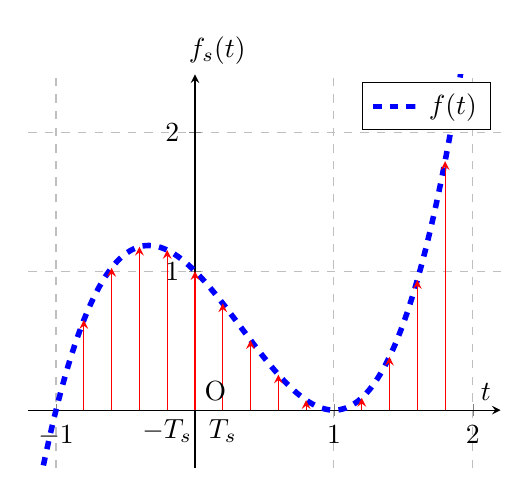
\begin{tikzpicture}
            \begin{axis}[
                axis lines = middle,
                xlabel = {$t$},
                ylabel = {$f_s(t)$},
                ylabel style={at={(rel axis cs:0.4, 1)}, anchor=south},
                xmin = -1.2, xmax = 2.2,
                ymin = -0.2, ymax = 2.2,
                xtick distance = 1,
                ytick distance = 1,
                grid = major,
                grid style = dashed,
                scale only axis,
                width = 6cm,
                height = 5cm,
                axis equal,
            ]
            \addplot[domain=-2.2:2.2, samples=100, smooth, line width=2pt, blue, dashed] {(x - 1)^2 * (x + 1)};
            \addlegendentry{$f(t)$}
            \draw[-stealth, smooth, red] (axis cs:-0.8, 0) -- (axis cs:-0.8, 0.648);
            \draw[-stealth, smooth, red] (axis cs:-0.6, 0) -- (axis cs:-0.6, 1.024);
            \draw[-stealth, smooth, red] (axis cs:-0.4, 0) -- (axis cs:-0.4, 1.176);
            \draw[-stealth, smooth, red] (axis cs:-0.2, 0) -- (axis cs:-0.2, 1.152);
            \draw[-stealth, smooth, red] (axis cs:0, 0) -- (axis cs:0, 1);
            \draw[-stealth, smooth, red] (axis cs:0.2, 0) -- (axis cs:0.2, 0.768);
            \draw[-stealth, smooth, red] (axis cs:0.4, 0) -- (axis cs:0.4, 0.504);
            \draw[-stealth, smooth, red] (axis cs:0.6, 0) -- (axis cs:0.6, 0.256);
            \draw[-stealth, smooth, red] (axis cs:0.8, 0) -- (axis cs:0.8, 0.072);
            \draw[-stealth, smooth, red] (axis cs:1.2, 0) -- (axis cs:1.2, 0.088);
            \draw[-stealth, smooth, red] (axis cs:1.4, 0) -- (axis cs:1.4, 0.384);
            \draw[-stealth, smooth, red] (axis cs:1.6, 0) -- (axis cs:1.6, 0.936);
            \draw[-stealth, smooth, red] (axis cs:1.8, 0) -- (axis cs:1.8, 1.792);
            \node at (axis cs:0, 0) [anchor=south west] {O};
            \node at (axis cs:-0.2, 0) [anchor=north] {$-T_s$};
            \node at (axis cs:0.2, 0) [anchor=north] {$T_s$};
            \end{axis}
        \end{tikzpicture}
        \caption{抽样信号}
        \label{fig:sampling-signal}
    \end{figure}
\end{example}

\begin{note}
    冲击信号、冲激串和抽样信号之间的关系如图 \ref{fig:impulse-impulse-train-sampled-signal} 所示:
    \begin{figure}[H]
        \centering
        \begin{tikzpicture}
            \node (impulse) [draw, rectangle, minimum width=2cm, minimum height=1cm] at (0, 0) {冲激信号};
            \node (impulse_train) [draw, rectangle, minimum width=2cm, minimum height=1cm] at (5, 0) {冲激串};
            \node (continuous_signal) [draw, rectangle, minimum width=2cm, minimum height=1cm] at (10, 0) {连续信号};
            \node (sampled_signal) [draw, rectangle, minimum width=2cm, minimum height=1cm] at (7.5, -2.5) {抽样信号};
        
            \draw[->, dashed, red] (impulse) -- node[above] {加法} (impulse_train);
            \draw[-] (continuous_signal) -- (impulse_train);
            \draw[->, dashed, red] (7.5, 0) -- node[right, pos=0.5] {乘法} (sampled_signal);
        \end{tikzpicture}
        \caption{冲击信号、冲激串和抽样信号之间的关系}
        \label{fig:impulse-impulse-train-sampled-signal}
    \end{figure}
\end{note}
